%! Author = adnansiddiquei
%! Date = 20/12/2023

\subsection{Q4 - Baseline Dataset}\label{subsec:q4}
\subsubsection{Question 4a}\label{subsubsec:q4a}
    Classification decision trees utilise recursive binary splitting to split the feature-space into high dimensional
    rectangles.
    Each iteration splits a rectangle into two, based on a feature and a threshold.
    The final tree has $N_{n}$ internal nodes, and $N_{n} + 1$ terminal nodes which represent the final classification:
    the modal class in that rectangle.
    Splits are assessed using criteria like the Gini index, choosing splits and thresholds that most reduce it.
    The Gini index \cite{ISL}, is:
    \begin{equation}
        G = \sum_{k=1}^{K} \hat{p}_{mk}(1 - \hat{p}_{mk})
        \label{eq:gini-index}
    \end{equation}
    where $\hat{p}_{mk}$ is the proportion of training samples in the $m$th region that are from the $k$th class.
    A region $m$ that contains mainly a single class will have a small Gini index for that region.

    Decision trees exhibit high variance.
    Ensemble methods like bagging and random forests reduce this variance.
    Bagging trains multiple trees on bootstrapped training data, with classifications decided by majority vote.
    Random forests further lower variance by randomly selecting features for each internal node split, creating less
    correlated trees.

    Two key hyperparameters in random forests are \inlinecode{max_depth} and \inlinecode{max_features}: the maximum
    internal nodes per tree and the number of features considered for splitting, respectively.
    Typically, \inlinecode{max_features} is set heuristically to $\sqrt{N}$, with $N$ being the feature count.

\subsubsection{Question 4b, 4c, 4d and 4e}\label{subsubsec:q4bcde}
    The dataset underwent preprocessing with the outlier removal method from Q3 (Section \ref{subsec:dataset-c}), followed by
    standardisation.
    It had no duplicates or missing values.
    Due to imbalanced classes, stratified sampling was employed for train-test splitting.

    \begin{figure}[htb]
    \centering
    \begin{subfigure}{0.5\textwidth}
        \centering
        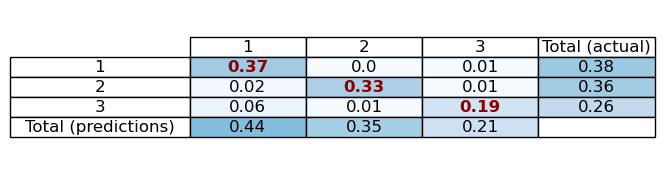
\includegraphics[width=0.9\textwidth]{./figures/q4c_confusion_matrix}
        \caption{Mean confusion matrix.}
        \label{fig:q4c_confusion_matrix}
    \end{subfigure}%
    \begin{subfigure}{0.5\textwidth}
        \centering
        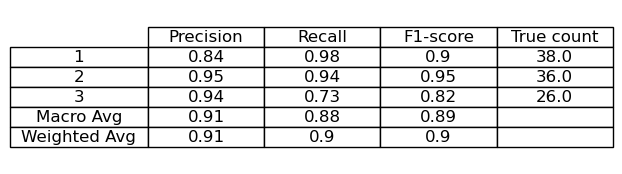
\includegraphics[width=0.9\textwidth]{./figures/q4c_classification_report}
        \caption{Mean classification report.}
        \label{fig:q4c_classification_report}
    \end{subfigure}
    \caption{The confusion matrix and classification report averaged over 5-fold cross-validation for
        \inlinecode{ADS_baselineDataset.csv} using a random forest classifier.
        The leading diagonal show a mean 10.0\% test set error.
        Matrix cells in (a) represent mean percentage allocations of the 100-sample test set, derived from a 0.8/0.2
        train-test split.}
    \label{fig:q4c}
    \end{figure}

    The dataset was then classified using \inlinecode{RandomForestClassifier} and Fig.\eqref{fig:q4c} shows a summary
    of the model performance.
    This gave a test set classification error of 10.0\%.

    \begin{figure}[htb]
    \centering
    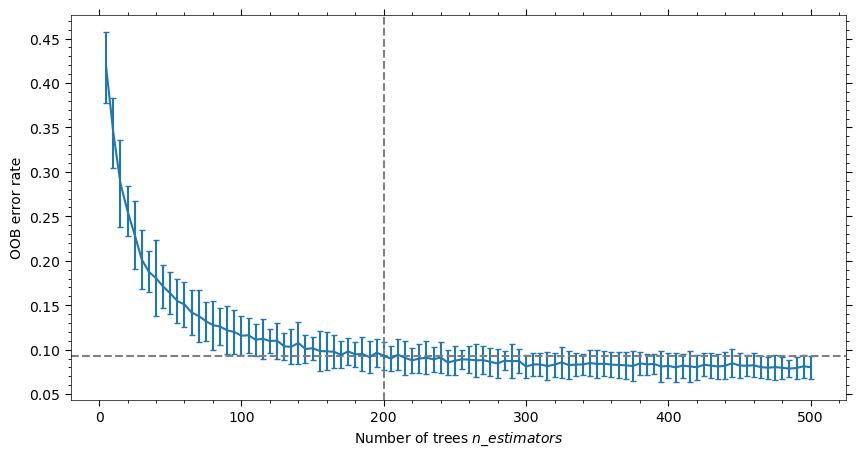
\includegraphics[width=0.9\textwidth]{./figures/q4d}
    \caption{The out of bag error rate for a \inlinecode{RandomForestClassifier} on the pre-processed dataset
        \inlinecode{ADS_baselineDataset.csv}. The OOB error rate was computed 20 times per
        \inlinecode{n_estimators} to give error bars.}
        \label{fig:q4d}
    \end{figure}

    \begin{figure}[htb]
    \centering
    \begin{subfigure}{0.5\textwidth}
        \centering
        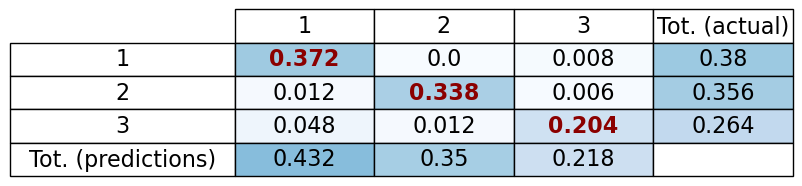
\includegraphics[width=0.9\textwidth]{./figures/q4d_confusion_matrix_200_trees}
        \caption{Mean confusion matrix.}
        \label{fig:q4d_confusion_matrix_200_trees}
    \end{subfigure}%
    \begin{subfigure}{0.5\textwidth}
        \centering
        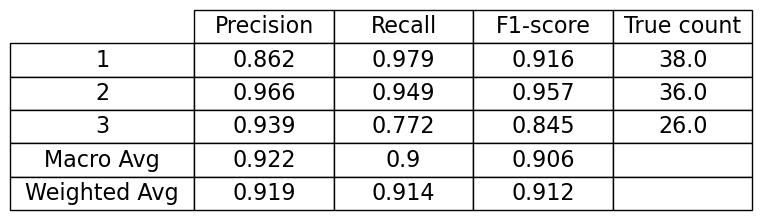
\includegraphics[width=0.9\textwidth]{./figures/q4d_classification_report_200_trees}
        \caption{Mean classification report.}
        \label{fig:q4d_classification_report_200_trees}
    \end{subfigure}
    \caption{Similar confusion matrix and classification reports as shown in Fig. \eqref{fig:q4c}, but with 200 trees.
        The mean test set classification error was 8.6\%.}
    \label{fig:q4d_200_trees}
    \end{figure}

    The \inlinecode{RandomForestClassifier} was then optimised based on the out-of-bag (OOB) error rate.
    Results in Fig. \eqref{fig:q4d} indicate that post 200 trees, the OOB error rate ceases to decrease significantly.
    Fig. \eqref{fig:q4d_200_trees} summarises model performance with 200 trees, showing the test set classification error
    improved to 8.6\% and improvements in average precision, recall, and F1-scores.

    \begin{figure}[htb]
    \centering
    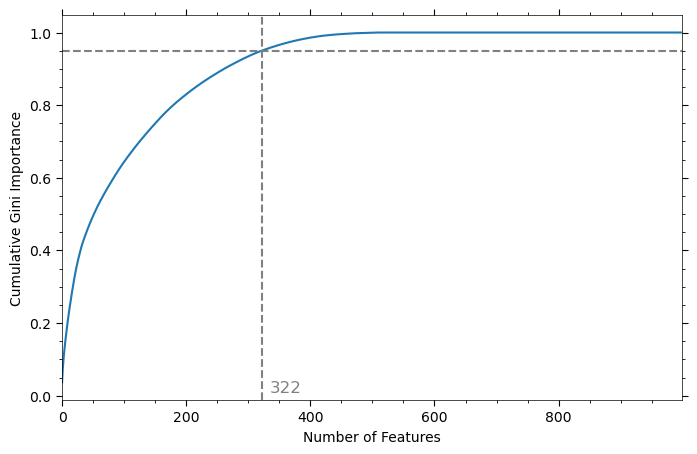
\includegraphics[width=0.9\textwidth]{./figures/q4e_gini_importance}
    \caption{The ordered (highest first), cumulative Gini importance of the features in
        \inlinecode{ADS_baselineDataset.csv}. The horizontal grey line is the 95\% threshold, which contains the top
        322 features.}
        \label{fig:q4e_gini_importance}
    \end{figure}

    \begin{figure}[htb]
    \centering
    \begin{subfigure}{0.5\textwidth}
        \centering
        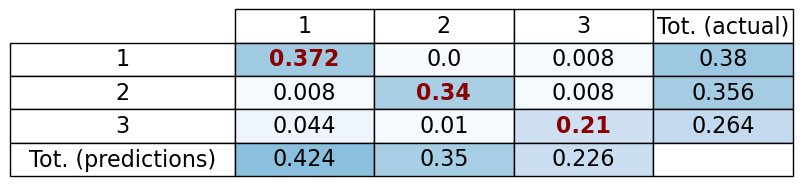
\includegraphics[width=0.9\textwidth]{./figures/q4e_confusion_matrix}
        \caption{Mean confusion matrix.}
        \label{fig:q4e_confusion_matrix}
    \end{subfigure}%
    \begin{subfigure}{0.5\textwidth}
        \centering
        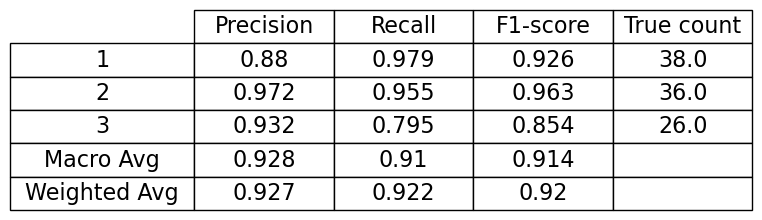
\includegraphics[width=0.9\textwidth]{./figures/q4e_classification_report}
        \caption{Mean classification report.}
        \label{fig:q4e_classification_report}
    \end{subfigure}
    \caption{Similar confusion matrix and classification reports as shown in Fig. \eqref{fig:q4c} and Fig. \eqref{fig:q4d_200_trees}
        but with 200 trees and utilising only the top 322 features. The mean test set classification error was 7.8\%.}
    \label{fig:q4e}
    \end{figure}

    \inlinecode{RandomForestClassifier.feature_importances_} was used to calculate Gini importance (Fig.
    \eqref{fig:q4e_gini_importance}).
    Gini importance measures the total normalised decrease in the Gini index due to internal splits on a feature.
    The top 322 features, representing 95\% of cumulative Gini importance, were selected for re-classification
    (see Fig. \eqref{fig:q4e}).
    Comparing Fig. \eqref{fig:q4d_200_trees} and Fig. \eqref{fig:q4e}, results were marginally better with the
    reduced feature set across all metrics

\subsubsection{Question 4f}\label{subsubsec:qf}
    \begin{figure}[htb]
    \centering
    \begin{subfigure}{0.5\textwidth}
        \centering
        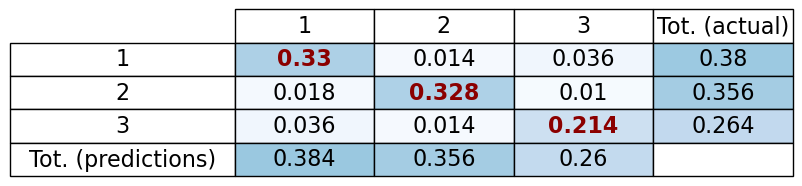
\includegraphics[width=0.9\textwidth]{./figures/q4f_confusion_matrix_all_feats}
        \caption{Mean confusion matrix.}
        \label{fig:q4f_confusion_matrix_all_feats}
    \end{subfigure}%
    \begin{subfigure}{0.5\textwidth}
        \centering
        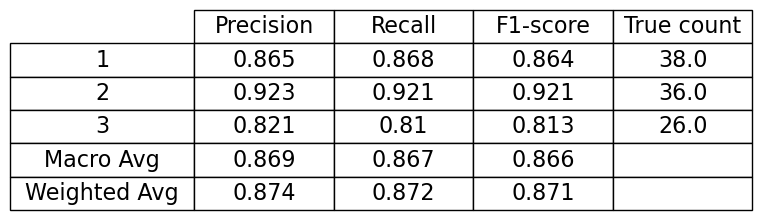
\includegraphics[width=0.9\textwidth]{./figures/q4f_classification_report_all_feats}
        \caption{Mean classification report.}
        \label{fig:q4f_classification_report_all_feats}
    \end{subfigure}
    \caption{Confusion matrix and classification report averaged over 5-folds of cross validation for the
        \inlinecode{LogisticRegression} classifier on \inlinecode{ADS_baselineDataset.csv}.
        The leading diagonal of the confusion matrix indicates a mean 12.8\% test set classification error.
        Matrix cells in (a) represent mean percentage allocations of the 100-sample test set, derived from a 0.8/0.2
        train-test split.}
    \label{fig:q4f_all_feats}
    \end{figure}

    \begin{figure}[htb]
    \centering
    \begin{subfigure}{0.5\textwidth}
        \centering
        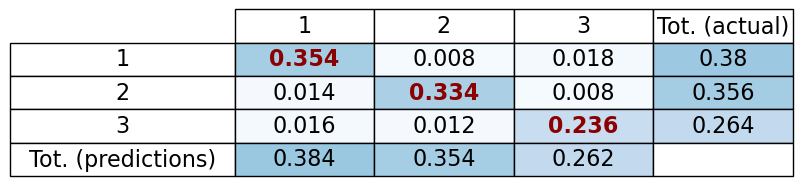
\includegraphics[width=0.9\textwidth]{./figures/q4f_confusion_matrix_reduced_feats}
        \caption{Mean confusion matrix.}
        \label{fig:q4f_confusion_matrix_reduced_feats}
    \end{subfigure}%
    \begin{subfigure}{0.5\textwidth}
        \centering
        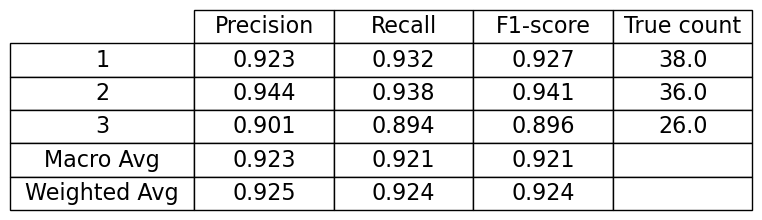
\includegraphics[width=0.9\textwidth]{./figures/q4f_classification_report_reduced_feats}
        \caption{Mean classification report.}
        \label{fig:q4f_classification_report_reduced_feats}
    \end{subfigure}
    \caption{Similar confusion matrix and classification reports as shown in Fig. \eqref{fig:q4f_all_feats} but with only
        the top 382 features. The mean test set classification error was 7.6\%.}
    \label{fig:q4f_reduced_feats}
    \end{figure}

    \begin{figure}[htb]
    \centering
    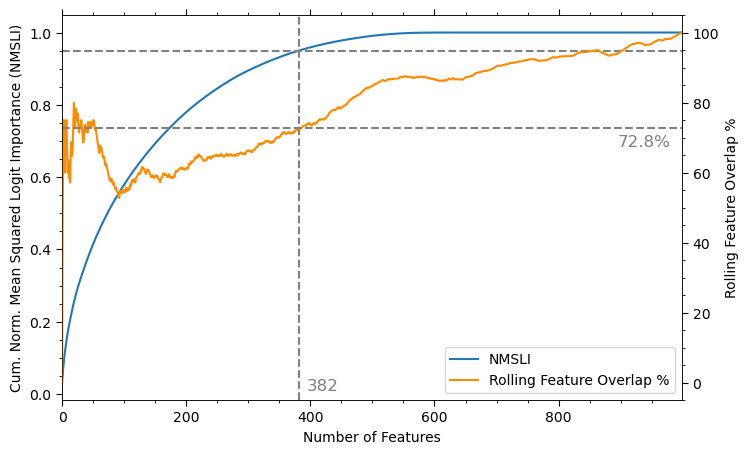
\includegraphics[width=0.9\textwidth]{./figures/q4f_logit_importance}
    \caption{The ordered (highest first), cumulative NMSLI of the features in the \inlinecode{LogisticRegression} model.
        The top horizontal grey line is the 95\% threshold, which contains the top 382 features. 72.8\% of these 382 features
        were also in the top 382 features for the \inlinecode{RandomForestClassifier} indicated by the Gini importance
        (Fig. \eqref{fig:q4e_gini_importance}) this is what the rolling feature overlap indicates.}
        \label{fig:q4f_logit_importance}
    \end{figure}

    The procedures outlined the previous section (Sec.\eqref{subsubsec:q4bcde}) were replicated using a multinomial logistic regression
    classifier, \inlinecode{LogisticRegression}.
    Fig.\eqref{fig:q4f_all_feats} and Fig.\eqref{fig:q4f_reduced_feats} illustrate the classification results using all
    features and the top 382 features, respectively.
    The latter demonstrates notably improved performance in test set classification error, precision, recall, and F1-scores.
    Feature importance was gauged using a novel metric, the normalised mean squared logit importance (NMSLI), calculated
    by averaging the squared coefficients for each feature across all 3 classes (\inlinecode{LogisticRegression.coef_}) and
    normalising them.
    This metric reflects the coefficient's magnitude and consistency across all classes, and was then treated like the
    Gini importance and the top 382 features were identified by calculating the features that contributed to 95\% of the
    cumulative NMSLI (Fig.\eqref{fig:q4f_logit_importance}).
    A comparison of Fig.\eqref{fig:q4e} and Fig.\eqref{fig:q4f_reduced_feats} shows similar performance across all
    metrics for both reduced feature-set \inlinecode{RandomForestClassifier} and \inlinecode{LogisticRegression} models.
